\section{Frequently Asked Questions}
\label{sec:FAQ}
This section shows frequently recurring problems, their cause, and a solution to solve them. First, in Section \ref{sec:Compilation Errors} we present solutions for errors occurring during the compilation. Section \ref{sec:Testing Errors} shows problems and solutions for errors, which may occur in testing.
\subsection{Errors while compiling}
This sections explains how build script errors can be resolved, which may appear while compiling projects and their plug-ins.
\label{sec:Compilation Errors}
\subsubsection{Compile failed}
\label{sec:Compile failed}
\begin{description}
	\item[Description] $ $\\
		The compilation target (\texttt{javac}) failed with an error message as shown below:
		\small$ $\\
			\verb|    ...|\\
			\verb|    [javac] <path>\<class file>:88: error: cannot find symbol|\\ 
			\verb|    [javac]         public void method(|\color{red}\verb|<a class>|\color{black}\verb| instance) {|\\
			\verb|    [javac]                               ^|\\
			\verb|    [javac]   symbol:   class |\color{red}\verb|<a class>|\color{black}\\
			\verb|    [javac]   location: class <class file>|\\
			\verb|    [javac] <path>\<class file>:33: error: |\color{red}\verb|<some.package>|\color{black}\verb| does not exist|\\
			\verb|    [javac] 		import |\color{red}\verb|<some.package>|\color{black}\verb|.<a class>);|\\
			\verb|    [javac]                          ^|\\
			\verb|    [javac] <path>\<class file>:77: error: cannot find symbol|\\
			\verb|    [javac] 			return new |\color{red}\verb|<class name>|\color{black}\verb|();|\\
			\verb|    [javac] 			                 ^|\\
			\verb|    [javac]   symbol:   class |\color{red}\verb|<class name>|\color{black}\\
			\verb|    [javac]   location: package <some.package>|\\
			\verb|    [javac] 9 errors|\\
			\verb|    [javac] 1 warning|\\
			\verb|    |\\
			\verb|BUILD FAILED|\\
			\verb|<project path>\build.xml:71: The following error occurred while executing|\\
			\verb| this line:|\\
			\verb|<plug-in path>build-jk.xml:40: Compile failed; see the compiler error|\\
			\verb| output for details.|\\
		\normalsize
	\item[Cause] $ $\\
	The plug-in defining the missing classes and packages is not added correctly to the \texttt{includes} path element at the beginning of the file (c.f. Figure \vref{lst:Build script of the IVML Editor}). This can have multiple reasons:
	\begin{enumerate}
		\item The related plug-in is not added to the \texttt{includes} path element.
		\item Some of the properties used inside the path element are pointing to the wrong location.
	\end{enumerate}
	\item[Solution] $ $
	\begin{enumerate}
		\item Add the necessary plug-ins to the \texttt{includes} path element as described in Section \ref{sec:Managing Plug-in Dependencies}.
		\item Check whether the properties are pointing to the correct locations, i.e. where the plug-in jars are created. You can add the following code at the beginning of the \texttt{compile} target to see the current content of the \texttt{includes} path element\footnote{cf. comment by Alfonso Phocco at \url{http://www.jguru.com/faq/view.jsp?EID=471917}}:\\
		  \verb|echo message="${toString:includes}"|\\
		The printed result must not contain any ant variables in the form of\\
		\color{red}\verb|${|\color{black}\verb|<a property name>|\color{red}\verb|}|\color{black}.\\
		You should also verify whether the properties of the \texttt{global-build.properties} are pointing to the correct location. The \texttt{libs} properties should point to the created jar file inside the corresponding project, i.e. \texttt{home} property. For instance:\\
		\color{red}\verb|libs.model|\color{black}\verb|=${home.|\color{red}\verb|model.dir|\color{black}\verb|}/${build.jar.dir}/...varModel.jar|
	\end{enumerate}
\end{description}
\newpage
\subsection{Errors while testing}
\label{sec:Testing Errors}
\subsubsection{Could not find plug-in}
\label{sec:Could not find plug-in}
\begin{description}
	\item[Description] $ $\\
		The automated test of the plug-in crashes with an error message as shown below:
		\footnotesize
			\verb|org.eclipse.test.EclipseTestRunner$TestFailedException:|\\
			\color{red}\verb|java.lang.Exception: Could not find plugin "de.uni-hildesheim.sse.<test plug-in name>"|\\
			\color{black}\verb|    at org.eclipse.test.EclipseTestRunner.runFailed(EclipseTestRunner.java:435)|\\
			\verb|    at ...|
		\normalsize
	\item[Cause] $ $\\
	The test plug-in could not be loaded by Eclipse. This means that either the test plug-in itself or one of the used plug-ins was not copied into the Eclipse test environment.
	\item[Solution] $ $\\
	Find the missing plug-ins and add them to the \texttt{copy.to.eclipse} target (see Figure \vref{lst:Adaption of build part 2}, lines 32 - 35). The easiest way of doing so, is to run the build script for the complete project on a local machine, start the OSGi console of the Eclipse instance for testing, and try to load the test plug-in. This can be done as follows:
	\begin{enumerate}
		\item Open a console for the \textit{plug-in}'s folder of the Eclipse instance for testing. After running the build script, the Eclipse instance is located at the \texttt{testEclipse} folder inside the \textit{project}'s folder.
		\item Open the OSGi console by running the command:\\
			\texttt{java -jar org.eclipse.equinox.launcher\_<version> -console}\\
			An example is given in Figure \vref{fig:Opening the OSGi console}.
			\begin{nofloat}{figure}
				\ifpdf	
				\begin{center}
				\hspace{-1.85cm}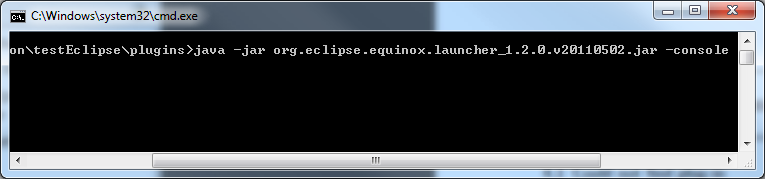
\includegraphics[width=\textwidth]{pictures/faq/OSGiConsole}
				\end{center}
				\fi
				\centering
				\caption[Opening the OSGi console]{Command for opening the OSGi console. This must be done inside the \textit{plug-in}'s folder of the Eclipse instance for testing after running the build script.}
				\label{fig:Opening the OSGi console}
			\end{nofloat}
			%\pic{0.75}{faq/OSGiConsole}{Opening the OSGi console}{Command for opening the OSGi console. This must be done inside the \textit{plug-in}'s folder of the Eclipse instance for testing after running the build script.}{Opening the OSGi console}
		\item Eclipse will ask for the workspace location. Ignore this window or accept it, but do not close the window as it will also stop the OSGi console.
		\item Run the command \texttt{ss} to list all installed OSGi bundles and search the test plug-in.
		\item If the plug-in is not listed, then install it with the command:\\
			\texttt{install file://<location>}\\
			Please note that you have to add a \texttt{\textbackslash} in front of the drive letter in Windows. An example is given in Figure \vref{fig:Installation of a Plug-in}.
			\begin{nofloat}{figure}
				\ifpdf	
				\hspace{-1.85cm}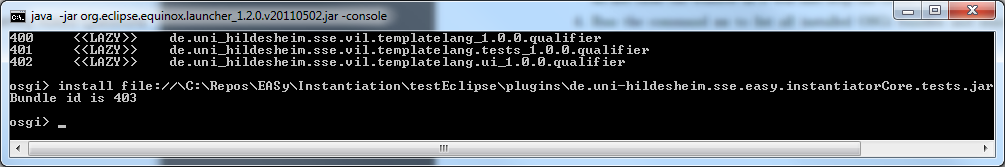
\includegraphics[width=\textwidth]{pictures/faq/installPlug-in}
				\fi
				\centering
				\caption[Installation of a plug-in]{Installation of a plug-in via the OSGi console. In Windows, you have to add a  \texttt{\textbackslash} in front of the drive letter.}
				\label{fig:Installation of a Plug-in}
			\end{nofloat}
		\item Try to load the bundle with running the command:\\
			\texttt{start <plug-in number>}\\
			This should fail, but the displayed error message will give you a hint, which plug-in is missing. Figure \vref{fig:Start Plug-in} shows the useful error message.
			\begin{nofloat}{figure}
				\ifpdf	
				\hspace{-1.85cm}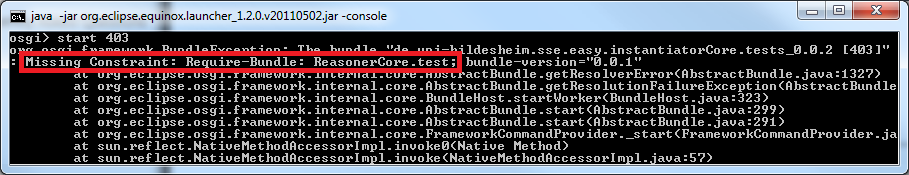
\includegraphics[width=\textwidth]{pictures/faq/startPlug-in}
				\fi
				\centering
				\caption[Failed attempt of starting a plug-in]{Failed attempt of starting a plug-in via the OSGi console. The error message shows that the \textit{ReasonerCore.tests} plug-in could not be started.}
				\label{fig:Start Plug-in}
			\end{nofloat}
		\item Check whether the crashing plug-in is located inside the \textit{plug-in}'s folder of the Eclipse instance for testing. Repeat the steps above, if the plug-in is located inside the \textit{plug-in}'s folder. Add the missing plug-in to the \texttt{copy.to.eclipse} target (see Figure \vref{lst:Adaption of build part 2}, lines 32 - 35).
	\end{enumerate}
\end{description}
\newpage
\subsubsection{java.lang.NoSuchMethodError: com.vladium.emma.rt.RT.S}
\label{sec:Emma Method Error}
\begin{description}
	\item[Description] $ $\\
		The automated test of the plug-in crashes with an error message as shown below:
		\small
			\verb|java.lang.NoSuchMethodError: |\color{red}\verb|com.vladium.emma.rt.RT.S([[ZLjava/lang/String;J)V|\\
			\color{black}\verb|    at de.uni_hildesheim.sse.parser.antlr.internal.InternalVilBuildLanguage...|\\
			\verb|    at ...|
		\normalsize
	\item[Cause] $ $\\
	The specified class was not instrumented correctly. This can have multiple reasons:
	\begin{enumerate}
		\item The Java file contains longer \texttt{static final String[]} definitions, which are not supported by Emma (cf. \url{http://sourceforge.net/p/emma/bugs/96/}).
	\end{enumerate}
	\item[Solution] $ $\\
	Depending on the cause, different solutions exist:	
	\begin{enumerate}
		\item In case a Java file contains longer \texttt{static final String[]} definitions, exclude this file from instrumentation. For this purpose, you have to add an exclusion filter to the \texttt{instrument} target (cf. Figure \vref{lst:Added exclusion filter}).
		\begin{nofloat}{figure}
			\centering
			\lstinputlisting[style=Plain, language=Ant, linerange={109 - 111, 115 - 115, 117 - 117, 133 - 136}]{\trunkDir/Instantiation/build.xml}
			\caption[Added exclusion filter to solve a com.vladium.emma.rt.RT.S error]{Modified Build script (\texttt{build.xml}) of the Instantiation project (excerpt). A new exclusion filter was specified in line 4 to exclude all Java classes of the \texttt{de.uni\_hildesheim.sse.parser.antlr.internal} package to avoid \texttt{java.lang.NoSuchMethodError: com.vladium.emma.rt.RT.S} error.}
			\label{lst:Added exclusion filter}
\end{nofloat}
	\end{enumerate}
\end{description}
\newpage
\subsubsection[java.lang.NoClassDefFoundError]{java.lang.NoClassDefFoundError: Could not initialize class <class name>}
\label{sec:NoClassDefFoundError}
\begin{description}
	\item[Description] $ $\\
		The automated test of the plug-in crashes with an error message as shown below:
		\small
			\verb|java.lang.NoClassDefFoundError: Could not initialize class |\color{red}\verb|<class name>|\\
			\color{black}\verb|    at java.lang.reflect.Constructor.newInstance(Constructor.java:525)|\\
			\verb|    at ...|
		\normalsize
	\item[Cause] $ $\\
	This problem has several possible causes:	
	\begin{enumerate}
		\item This problem is related with the problem described in Section \vref{sec:Emma Method Error}.
		\item This problem also appears if referenced libraries are not packed into the plug-in's jar file. In this case, \color{red}\texttt{<class name>}\color{black}\ should be the name of a third party class, e.g. \texttt{org/apache/commons/io/FilenameUtils}.
	\end{enumerate}
	\item[Solution] $ $
	\begin{enumerate}
		\item Solve the problem as described in Section \ref{sec:Emma Method Error}.
		\item Edit the \texttt{build-jk} file of the plug-in and add the \texttt{copy} task of Figure \vref{lst:Added necessary libraries} to the \texttt{jar} target.
		\begin{nofloat}{figure}
			\centering
			\lstinputlisting[style=Plain, language=Ant, linerange={49 -57}] {\trunkDir/Instantiation/de.uni_hildesheim.sse.vil.buildlang.tests/build-jk.xml}
			\caption[Creation of a jar, including referenced libraries]{Modified Build script (\texttt{build-jk.xml}) of \texttt{de.uni\_hildesheim.sse.vil.build\-lang.tests} plug-in (excerpt). The lines 3 -- 7 are added to include necessary libraries.}
			\label{lst:Added necessary libraries}
\end{nofloat}
	\end{enumerate}
\end{description}